\documentclass[11pt]{beamer}

\mode<presentation>
\usetheme{metropolis}

\usepackage{appendixnumberbeamer}
\usepackage{booktabs}
\usepackage[scale=2]{ccicons}
\usepackage{fontspec}
\usepackage{graphicx}

\usepackage{polyglossia}
\setdefaultlanguage[variant=brazil]{portuguese}

\usepackage{alltt}
\renewcommand{\ttdefault}{txtt}
\usepackage{xcolor}

\usefonttheme{professionalfonts}
\usepackage{fontspec}
\setsansfont{Fira Sans}
\setmonofont{Fira Mono}

\setbeamertemplate{frame footer}{\href{http://creativecommons.org/licenses/by-sa/4.0/}{\ccbysa}
                                 \footnotesize{ \url{https://github.com/ayharano/just-python/}}}

\graphicspath{ {.} }


\title{\normalsize{Comprehensions: ler, entender e utilizar}}
\author{\href{https://alexandre.harano.net.br/}{Alexandre Yukio Harano}}
\institute[.]
{alexandre@harano.net.br\\
 \url{https://alexandre.harano.net.br/}}
\date{\scriptsize{\href{https://pythonsul.org/}{Curitiba, 12 de Setembro de 2019}
 --
\href{https://pythonsul.org/}{Python Sul}}}



\begin{document}

\maketitle

\begin{frame}[standout]
  O que é \textit{comprehension}?
\end{frame}

\begin{frame}[fragile]{Comprehension}
  \begin{flushright}
  \begin{minipage}{\linewidth}\begin{flushleft}
  Uma maneira compacta de processar todos os ou parte dos elementos de uma sequência e devolver (uma~lista | um~dicionário | um~conjunto) com os resultados.
  \end{flushleft}
  \end{minipage}

  \tiny{\vspace*{.25cm}
    Adaptado de \url{https://docs.python.org/3/glossary.html#term-list-comprehension}}
  \end{flushright}
\end{frame}

\begin{frame}[fragile]{Comprehension}
  \begin{flushright}
  \begin{alltt}\small
\textbf{comprehension} ::=  \textcolor{blue}{expression} \textcolor{blue}{comp_for}
\textbf{comp_for}      ::=  ["async"] "for" \textcolor{blue}{target_list} "in"
                   \textcolor{blue}{or_test} [\textcolor{blue}{comp_iter}]
\textbf{comp_iter}     ::=  \textcolor{blue}{comp_for} | \textcolor{blue}{comp_if}
\textbf{comp_if}       ::=  "if" \textcolor{blue}{expression_nocond} [\textcolor{blue}{comp_iter}]
\end{alltt}

  \tiny{\vspace*{.25cm}
    Extraído de \url{https://docs.python.org/3/reference/expressions.html#list-displays}}
  \end{flushright}
\end{frame}

\begin{frame}[fragile]{( List | Dict | Set ) Comprehensions}
  \begin{overprint}
  Expressivo mecanismo para criação de uma nova instância de lista/dicionário/conjunto.\only<2->{.}\only<3->{.}\only<4->{ se usado cautelosamente.}
  \end{overprint}
\end{frame}

\begin{frame}[fragile]{( List | Dict | Set ) Comprehensions}
  \begin{alltt}\scriptsize
lista = [
    \textcolor{blue}{EXPRESSÃO_DO_CONTEÚDO}
    "for" ... "in" ...
    "if" ...
]

dicionário = \{
    \textcolor{blue}{EXPRESSÃO_DA_CHAVE}: \textcolor{blue}{EXPRESSÃO_DO_VALOR} 
    "for" ... "in" ...
    "if" ...
\}

conjunto = \{
    \textcolor{blue}{EXPRESSÃO_DO_VALOR} 
    "for" ... "in" ...
    "if" ...
\}
\end{alltt}
\end{frame}

\begin{frame}[fragile]{( List | Dict | Set ) Comprehensions}
  Aloca os recursos necessários para \textbf{todos} os elementos que atendam os critérios.
\end{frame}

\begin{frame}[fragile]{Expressão Geradora}
  \begin{alltt}\scriptsize
expressão_geradora = (
    \textcolor{blue}{EXPRESSÃO_DO_CONTEÚDO}
    "for" ... "in" ...
    "if" ...
)
\end{alltt}
\end{frame}

\begin{frame}[fragile]{Expressão Geradora}
  Aloca os recursos necessários \textbf{item a item conforme demanda}.
\end{frame}

\begin{frame}[fragile]{Por que Expressão Geradora e não Generator Comprehension?}
  \begin{flushright}
  \begin{minipage}{\linewidth}\begin{flushleft}
\textbf{Resposta}:

\emph{Comprehensions} foram pensados inicialmente para \emph{aparentar} com as estruturas de dados construídas (termo original: \emph{display}) e \emph{geradores} não possuem tal relação.
  \end{flushleft}
  \end{minipage}

  \tiny{\vspace*{.25cm}
     Mais detalhes em \url{https://nedbatchelder.com/blog/201605/generator_comprehensions.html}}
  \end{flushright}
\end{frame}

\begin{frame}[fragile]{Um Pequeno Desvio...}
  \begin{alltt}\small
>>> lista = [x for x in range(0)]
>>> lista
[]
>>> bool(lista)
False

>>> expressão_geradora = (x for x in range(0))
>>> expressão_geradora
<generator object <genexpr> at 0x7f4ee64f9bf8>
>>> bool(expressão_geradora)
True
\end{alltt}
\end{frame}

\begin{frame}[fragile]{... E Como Contornar}
  \begin{alltt}\small
>>> expressão_geradora = (x for x in range(0))
>>> expressão_geradora
<generator object <genexpr> at 0x7f4ee64f9bf8>
>>> bool(expressão_geradora)
True

>>> lista_da_expressão_geradora =
...     list(expressão_geradora)
>>> lista_da_expressão_geradora
[]
>>> bool(lista_da_expressão_geradora)
False
\end{alltt}
\end{frame}

\begin{frame}[fragile]{Iteradores Com Variáveis Dependentes}
  Iterações são lidas da expressão mais a esquerda para a direita.

\vfill

\begin{minipage}{0.4\linewidth}
  Exemplo:
  \begin{alltt}\footnotesize
>>> matriz_triangular_3x3 = [
...     (x, y)
...     for y in range(3)
...     for x in range(y+1)
... ]
>>> matriz_triangular_3x3
[(0, 0), (0, 1), (1, 1),
 (0, 2), (1, 2), (2, 2)]
\end{alltt}
\end{minipage}
\hfill
\begin{minipage}{0.4\linewidth}
   \centering{
\includegraphics[width=0.9\linewidth]{3x3}}
\end{minipage}
\end{frame}

\begin{frame}[fragile]{\href{https://www.python.org/dev/peps/pep-0530/}{Asynchronous Comprehensions (PEP 530)}}
  \begin{itemize}
    \item Só pode ser utilizado dentro de funções com \texttt{async def}.
    \item Expressões podem ser calculadas a partir de
    \begin{enumerate}[i]
      \item Iteradores assíncronos (\texttt{expr async for ...}); ou
      \item Uso de \texttt{await} em \emph{comprehensions} regulares (\texttt{await expr for ...}).
    \end{enumerate}
  \end{itemize}
\end{frame}


\begin{frame}[standout]
  Análise de código
\end{frame}

\begin{frame}[fragile]{\href{https://docs.python.org/3/library/dis.html}{\texttt{dis}}}
   \hspace*{-.5cm}\centering{\href{https://docs.python.org/3/library/dis.html}{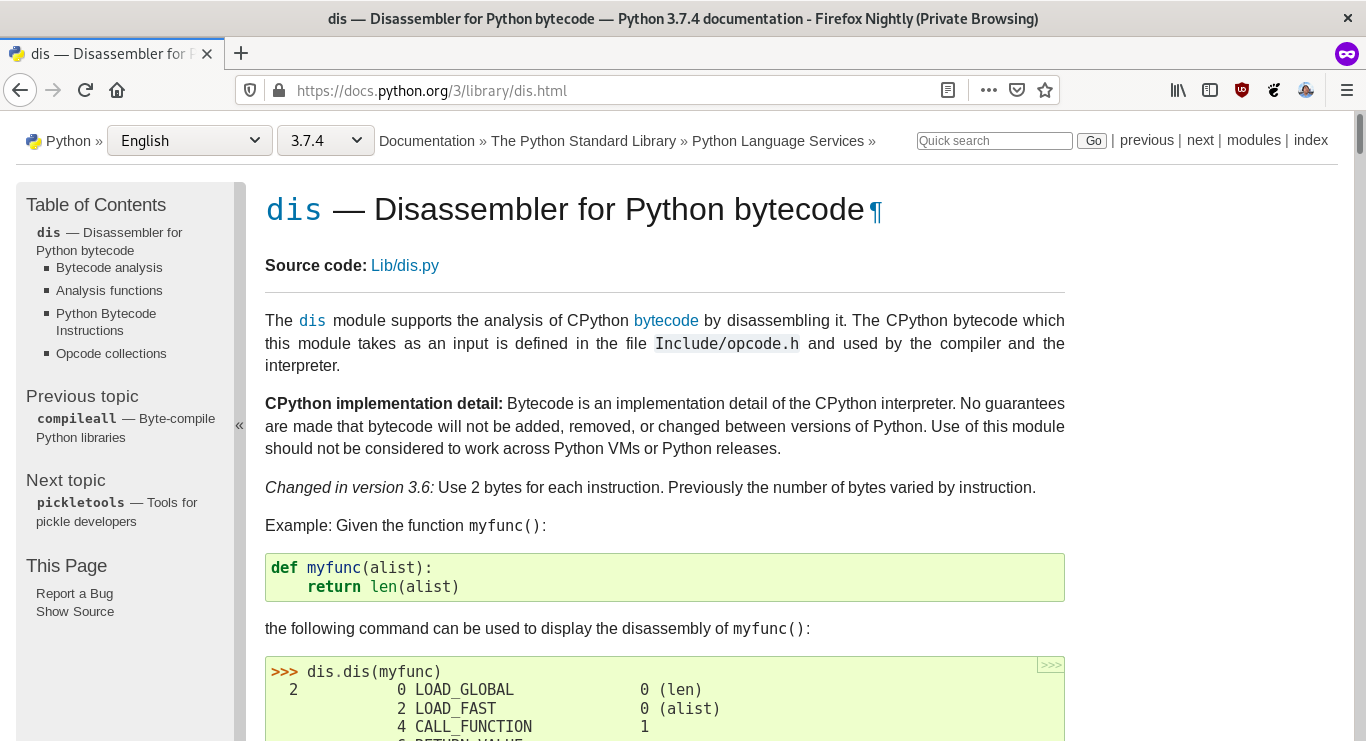
\includegraphics[width=12cm]{dis}}}
\end{frame}

\begin{frame}[fragile]{\href{https://docs.python.org/3/library/dis.html}{\texttt{dis}}}
\begin{alltt}\small
>>> def via_nome(): return list()
>>> def via_símbolo(): return []

>>> import dis
>>> dis.dis(via_nome)
  1           0 LOAD_GLOBAL              0 (list)
              2 CALL_FUNCTION            0
              4 RETURN_VALUE
>>> dis.dis(via_símbolo)
  1           0 BUILD_LIST               0
              2 RETURN_VALUE
\end{alltt}
\end{frame}


\begin{frame}[fragile]{Comparação}
  \begin{alltt}\scriptsize
def usual():
    resultado = []
    for valor in range(100):
        if valor % 2:
            resultado.append(valor)
    return resultado

def list_comp():
    return [
        valor
        for valor in range(100)
        if valor % 2
    ]

def filter_lambda():
    return list(
        filter(lambda valor: valor % 2, range(100))
    )
\end{alltt}
\end{frame}

\begin{frame}[fragile]{Comparação (\texttt{usual})}
\vspace*{-.25cm}
  \begin{alltt}\tiny
>>> dis.dis(usual)
  2           0 BUILD_LIST               0
              2 STORE_FAST               0 (resultado)

  3           4 SETUP_LOOP              34 (to 40)
              6 LOAD_GLOBAL              0 (range)
              8 LOAD_CONST               1 (100)
             10 CALL_FUNCTION            1
             12 GET_ITER
        >>   14 FOR_ITER                22 (to 38)
             16 STORE_FAST               1 (valor)

  4          18 LOAD_FAST                1 (valor)
             20 LOAD_CONST               2 (2)
             22 BINARY_MODULO
             24 POP_JUMP_IF_FALSE       14

  5          26 LOAD_FAST                0 (resultado)
             28 LOAD_METHOD              1 (append)
             30 LOAD_FAST                1 (valor)
             32 CALL_METHOD              1
             34 POP_TOP
             36 JUMP_ABSOLUTE           14
        >>   38 POP_BLOCK

  6     >>   40 LOAD_FAST                0 (resultado)
             42 RETURN_VALUE
\end{alltt}
\end{frame}

\begin{frame}[fragile]{Comparação (\texttt{list\_comp})}
\vspace*{-.25cm}
  \begin{alltt}\tiny
>>> dis.dis(list_comp)
  3           0 LOAD_CONST               1 (<code object <listcomp> at 0x7fddefe4ced0, file "<stdin>", line 3>)
              2 LOAD_CONST               2 ('list_comp.<locals>.<listcomp>')
              4 MAKE_FUNCTION            0

  4           6 LOAD_GLOBAL              0 (range)
              8 LOAD_CONST               3 (100)
             10 CALL_FUNCTION            1
             12 GET_ITER
             14 CALL_FUNCTION            1
             16 RETURN_VALUE

Disassembly of <code object <listcomp> at 0x7fddefe4ced0, file "<stdin>", line 3>:
  3           0 BUILD_LIST               0
              2 LOAD_FAST                0 (.0)
        >>    4 FOR_ITER                16 (to 22)

  4           6 STORE_FAST               1 (valor)

  5           8 LOAD_FAST                1 (valor)
             10 LOAD_CONST               0 (2)
             12 BINARY_MODULO
             14 POP_JUMP_IF_FALSE        4
             16 LOAD_FAST                1 (valor)
             18 LIST_APPEND              2
             20 JUMP_ABSOLUTE            4
        >>   22 RETURN_VALUE
\end{alltt}
\end{frame}

\begin{frame}[fragile]{Comparação (\texttt{filter\_lambda})}
\vspace*{-.25cm}
  \begin{alltt}\tiny
>>> dis.dis(filter_lambda)
  2           0 LOAD_GLOBAL              0 (list)

  3           2 LOAD_GLOBAL              1 (filter)
              4 LOAD_CONST               1 (<code object <lambda> at 0x7efd64690a50, file "<stdin>", line 3>)
              6 LOAD_CONST               2 ('filter_lambda.<locals>.<lambda>')
              8 MAKE_FUNCTION            0
             10 LOAD_GLOBAL              2 (range)
             12 LOAD_CONST               3 (100)
             14 CALL_FUNCTION            1
             16 CALL_FUNCTION            2
             18 CALL_FUNCTION            1
             20 RETURN_VALUE

Disassembly of <code object <lambda> at 0x7efd64690a50, file "<stdin>", line 3>:
  3           0 LOAD_FAST                0 (valor)
              2 LOAD_CONST               1 (2)
              4 BINARY_MODULO
              6 RETURN_VALUE
\end{alltt}
\end{frame}


\begin{frame}[fragile]{Asynchronous Comprehensions}
\vspace*{-.25cm}
  \begin{alltt}\scriptsize
import asyncio


async def intervalo_progressivo(espera, até):
    for i in range(até):
        yield i
        await asyncio.sleep(espera)


async def async_set():
    return \{
        valor
        async for valor in intervalo_progressivo(.001, 100)
        if valor % 2
    \}
\end{alltt}
\end{frame}


\begin{frame}[fragile]{Asynchronous Comprehensions}
\vspace*{-.25cm}
  \begin{alltt}\tiny
>>> dis.dis(async_set)
 10           0 LOAD_CONST               1 (<code object <setcomp> at 0x7f4b340f0a50, file "async_set.py", line 10>)
              2 LOAD_CONST               2 ('async_set.<locals>.<setcomp>')
              4 MAKE_FUNCTION            0

 12           6 LOAD_GLOBAL              0 (intervalo_progressivo)
              8 LOAD_CONST               3 (0.001)
             10 LOAD_CONST               4 (100)
             12 CALL_FUNCTION            2
             14 GET_AITER
             16 CALL_FUNCTION            1
             18 GET_AWAITABLE
             20 LOAD_CONST               0 (None)
             22 YIELD_FROM
             24 RETURN_VALUE

...
\end{alltt}
\end{frame}

\begin{frame}[fragile]{Asynchronous Comprehensions}
\vspace*{-.25cm}
  \begin{alltt}\tiny
...

Disassembly of <code object <setcomp> at 0x7f4b340f0a50, file "async_set.py", line 10>:
 10           0 BUILD_SET                0
              2 LOAD_FAST                0 (.0)
        >>    4 SETUP_EXCEPT            12 (to 18)
              6 GET_ANEXT
              8 LOAD_CONST               0 (None)
             10 YIELD_FROM

 12          12 STORE_FAST               1 (valor)
             14 POP_BLOCK
             16 JUMP_FORWARD            10 (to 28)
        >>   18 DUP_TOP
             20 LOAD_GLOBAL              0 (StopAsyncIteration)
             22 COMPARE_OP              10 (exception match)
             24 POP_JUMP_IF_TRUE        42
             26 END_FINALLY

...
\end{alltt}
\end{frame}

\begin{frame}[fragile]{Asynchronous Comprehensions}
\vspace*{-.25cm}
  \begin{alltt}\tiny
...


 13     >>   28 LOAD_FAST                1 (valor)
             30 LOAD_CONST               1 (2)
             32 BINARY_MODULO
             34 POP_JUMP_IF_FALSE        4
             36 LOAD_FAST                1 (valor)
             38 SET_ADD                  2
             40 JUMP_ABSOLUTE            4
        >>   42 POP_TOP
             44 POP_TOP
             46 POP_TOP
             48 POP_EXCEPT
             50 POP_TOP
             52 RETURN_VALUE
\end{alltt}
\end{frame}


\begin{frame}[fragile]{Não-Exemplos (Aprecie Com Moderação!)}
  \begin{flushright}
  \begin{alltt}\scriptsize
  resultado = [transformação_complexa(
                x, algum_argumento=x+1)
               for x in iterável if predicado(x)]

  resultado = [
      (x, y)
      for x in range(10)
      for y in range(5)
      if x * y > 10
  ]

  return ((x, y, z)
          for x in range(5)
          for y in range(5)
          if x != y
          for z in range(5)
          if y != z)
\end{alltt}

  \tiny{\vspace*{.25cm}
    Adaptado de \url{https://github.com/google/styleguide/blob/gh-pages/pyguide.md}}
  \end{flushright}
\end{frame}

\begin{frame}[fragile]{Pontos principais}
  \begin{itemize}
    \item \emph{Comprehensions} são utilizados para \textbf{criar} listas|dicionários|conjuntos.
    \item Pode melhorar a legibilidade de código principalmente para filtrar dados.
    \item Variáveis alocadas dentro da \emph{comprehensions} só valem dentro do escopo local, ou seja, menos variáveis temporárias.
    \item Não recomendado usar com expressões que exijam tratamento (ex: \texttt{Exception}s).
    \item Cautela com os recursos! Se souber de antemão que os dados extrapolam a memória, usar \emph{expressões geradoras}.
  \end{itemize}
\end{frame}


\begin{frame}[standout]
  \vspace*{2cm}
  \huge{Perguntas?}
  \begin{block}{}
    \vspace*{2cm}
    \begin{flushright}
      \large{\href{https://alexandre.harano.net.br/}{Alexandre Yukio Harano}} \\ \vspace*{0.1cm}
      \small{\href{mailto:alexandre@harano.net.br}{alexandre@harano.net.br}} \\
      \small{\url{https://alexandre.harano.net.br/}}
    \end{flushright}
    \vspace*{.2cm}
    \begin{flushleft}
      \normalsize{\url{https://github.com/ayharano/just-python/}}
    \end{flushleft}
  \end{block}
\end{frame}

\end{document}
